\section{Runtime Architecture and Research Context}
\label{sec:runtime}
\subsection{Execution as a stateful transaction}
A speculative iteration advances a committed prefix through draft, target verification, and reconciliation. The draft proposes up to $k$ tokens. The target evaluates the pending token and proposal positions, often through a caller batch containing several tokens. Acceptance, correction, and a possible bonus token determine what is committed. Rejected positions must then be removed or reconciled before the next iteration. Stopping is evaluated under the registered EOG and cap rule. Figure~\ref{fig:architecture} locates the state interfaces and the four phase controls examined here.

The runtime state includes more than committed IDs. Target and draft KV ownership, logical positions, pending logits or tokens, sampler history, and loop counters connect successive calls. A pending token may already have been sampled and accepted into the sampler while remaining to be evaluated into the cache. A transfer that repeats or omits this event changes the transaction. Early intervention frontends therefore retain pending state and clone behavior as well as KV. The later B570 candidate instead binds phases in the same context and live sampler. The RTX cost candidate does not activate its optional state-transplant branch.

\begin{figure*}[t]
\centering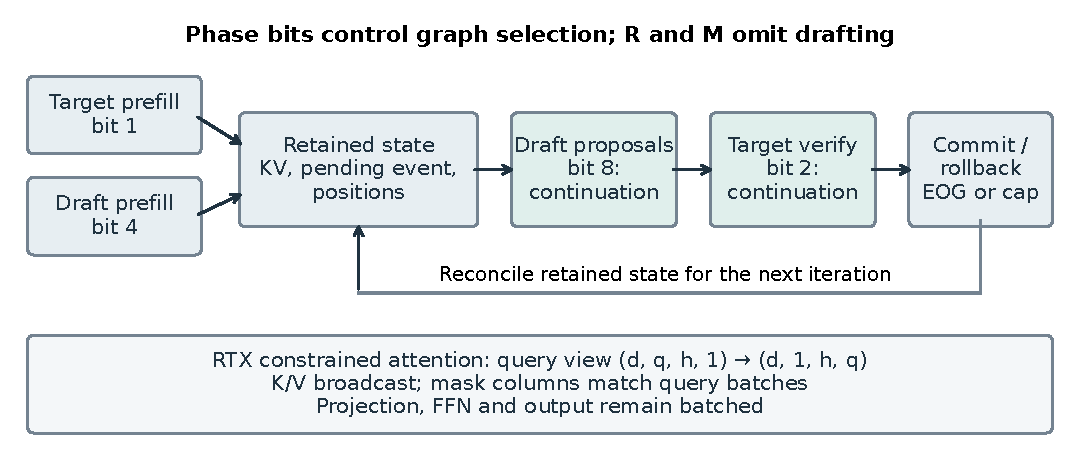
\includegraphics[width=\linewidth]{figures/figure_1_architecture.pdf}
\caption{Stateful execution and four phase controls: target prefill/continuation (bits 1/2), draft prefill/continuation (bits 4/8). Commit/rollback reconciles retained state. Ordinary $R$ and matched $M$ omit drafting. The source-bound, ChatGPT/Codex-assisted diagram does not imply active state transplantation in the RTX cost candidate.}
\label{fig:architecture}
\end{figure*}

The microbatch capacity, denoted UB, limits how a caller batch is partitioned for backend execution. It is distinct from $k$, occupied query count, and the number of output rows reserved by the frontend. UB2 can process a caller with one occupied continuation token. A larger $k$ can lower caller count while increasing the number of micrographs. Output reservation can change the recipe even at the same UB. These distinctions matter when interpreting a cross or a performance counter.

The native implementation is based on pinned llama.cpp releases and source-bound private frontends~\cite{llamacpp}. The late RTX graph uses Qwen3-8B as target and Qwen3-0.6B as draft~\cite{qwen3}, both Q8\_0, with non-flash CUDA attention. The intervention uses existing ggml views and operations; it adds neither a new CUDA arithmetic kernel nor a new acceptance rule. B570 uses Vulkan with a different frontend and phase-binding operation. Metal and OpenVINO-related historical cases retain their own runtime contracts. These are software execution choices on consumer hardware, rather than controlled comparisons of hardware alone.

\subsection{Reference preservation and prior determinism work}
The output requirement is deliberately narrower than general determinism. A token sequence can match while logits or cache values differ. Conversely, deterministic repetition of a candidate can stably reproduce the wrong reference. We register the ordinary path and endpoint before asking whether a transformation preserves them. Numerical consistency research already explains why shape-dependent reductions can alter such behavior. Batch-invariant inference constrains reduction strategies across batches~\cite{thinkingmachines}.

LLM-42 uses a decode--verify--rollback design, fixed verification shapes with padding, and replacement of decoded KV entries by verifier entries~\cite{llm42}. It also permits distinct consistent strategies for prefill and decode. Stage-Replay studies fixed-prefix precision controls and bidirectional cache transplantation~\cite{stagereplay}. Vosti specifies and verifies deterministic inference at a system level~\cite{vosti}. MarginGate uses margin-triggered verification and repairs confirmed mismatches~\cite{margingate}. These works establish principles that this manuscript uses rather than renames. Table~\ref{tab:related} states the specific additional evidence and the comparisons not performed.

\begin{table*}[t]\centering\small
\caption{Closest research context and the scope of this study. No row implies an implementation or speed advantage over the cited method.}
\label{tab:related}
\begin{tabularx}{\linewidth}{@{}p{.23\linewidth}XX@{}}\toprule
Prior work & Established basis & Additional evidence here\\\midrule
Batch-invariant inference; LLM-42~\cite{thinkingmachines,llm42} & Reduction/shape consistency; verified tokens and KV reconciliation & Qwen3 query views, phase dispatch and finite scope, followed by ordinary and matched paid costs\\
Stage-Replay; Vosti~\cite{stagereplay,vosti} & Fixed-prefix state intervention; specified system determinism & Natural donor $\times$ current recipe with shams; finite output qualification rather than a verified general guarantee\\
Consumer cost anatomy; Performance or Illusion?~\cite{lossless,illusion} & Backend verification cost and weak performance proxies & Reference-qualified fixed-UB width counterexample and distinction between target-path and speculative request gains\\\bottomrule
\end{tabularx}
\end{table*}

Natural crosses examine retained state and the current native recipe at a shared committed boundary. They motivate a candidate whose sufficiency requires native qualification. No same-contract implementation comparison with LLM-42, Stage-Replay or Vosti was performed.

\subsection{Performance and heterogeneous execution}
Heterogeneous placement and draft-budget control are established design directions. Dovetail and DuoDecoding exploit complementary CPU/GPU capabilities~\cite{dovetail,duodecoding}; TurboSpec and BanditSpec adapt speculation to execution conditions~\cite{turbospec,banditspec}. The published HeteroSpec studies contextual heterogeneity for verification allocation~\cite{aclheterospec}. Our title distinguishes the present reference-preservation question from that work.

Lossless but Not Free examines consumer backend cost, cache choreography, and cases in which verification fails to amortize target work~\cite{lossless}. Performance or Illusion? studies speculative decoding in a production engine and shows why apparent reductions in decoding work do not guarantee performance~\cite{illusion}. Here, output qualification, finite repair scope and ordinary versus matched paid baselines determine operating choices. Historical M4 and 358H results address control and offload limits under separate contracts; they do not replicate the RTX repair.
